\documentclass[12pt]{article}

%==============Packages & Commands==============
\usepackage{graphicx}
\usepackage{fancyvrb}
\usepackage{tikz}
%%%<
\usepackage{verbatim}
%\usepackage[active,tightpage]{preview}
%\PreviewEnvironment{tikzpicture}
%\setlength\PreviewBorder{5pt}%

\usepackage{geometry}                		% See geometry.pdf to learn the layout options. There are lots.
\geometry{letterpaper}                   		% ... or a4paper or a5paper or ...
%\geometry{landscape}                		% Activat\usetikzlibrary{arrows}e for for rotated page geometry
%\usepackage[parfill]{parskip}    		% Activate to begin paragraphs with an empty line rather than an indent
\usepackage{graphicx}				% Use pdf, png, jpg, or eps§ with pdflatex; use eps in DVI mode
								% TeX will automatically convert eps --> pdf in pdflatex
\usepackage{amssymb}

\usepackage[ruled,vlined]{algorithm2e}
\usetikzlibrary{arrows}
\usepackage{alltt}
\usepackage[T1]{fontenc}
\usepackage[utf8]{inputenc}
\usepackage{indentfirst}
\usepackage[longnamesfirst]{natbib} % For references
\bibpunct{(}{)}{;}{a}{}{,} % Reference punctuation
\usepackage{changepage}
\usepackage{setspace}
\usepackage{booktabs} % For tables
\usepackage{rotating} % For sideways tables/figures
\usepackage{amsmath}
\usepackage{multirow}
\usepackage{color}
\usepackage{dcolumn}
\usepackage{comment}
%\usepackage{fullwidth}
\newcolumntype{d}[1]{D{.}{\cdot}{#1}}
\newcolumntype{.}{D{.}{.}{-1}}
\newcolumntype{3}{D{.}{.}{3}}
\newcolumntype{4}{D{.}{.}{4}}
\newcolumntype{5}{D{.}{.}{5}}
\usepackage{float}
\usepackage[hyphens]{url}
%\usepackage[margin = 1.25in]{geometry}
%\usepackage[nolists,figuresfirst]{endfloat} % Figures and tables at the end
\usepackage{subfig}
\captionsetup[subfloat]{position = top, font = normalsize} % For sub-figure captions
\usepackage{fancyhdr}
%\makeatletter
%\def\url@leostyle{%
%  \@ifundefined{selectfont}{\def\UrlFont{\sf}}{\def\UrlFont{\small\ttfamily}}}
%\makeatother
%% Now actually use the newly defined style.
\urlstyle{same}
\usepackage{times}
\usepackage{mathptmx}
%\usepackage[colorlinks = true,
%						bookmarksopen = true,
%						pagebackref = true,
%						linkcolor = black,
%						citecolor = black,
% 					urlcolor = black]{hyperref}
%\usepackage[all]{hypcap}
%\urlstyle{same}
\newcommand{\fnote}[1]{\footnote{\normalsize{#1}}} % 12 pt, double spaced footnotes
\def\citeapos#1{\citeauthor{#1}'s (\citeyear{#1})}
\def\citeaposs#1{\citeauthor{#1}' (\citeyear{#1})}
\newcommand{\bm}[1]{\boldsymbol{#1}} %makes bold math symbols easier
\newcommand{\R}{\textsf{R}\space} %R in textsf font
\newcommand{\netinf}{\texttt{NetInf}\space} %R in textsf font
\newcommand{\iid}{i.i.d} %shorthand for iid
\newcommand{\cites}{{\bf \textcolor{red}{CITES}}} %shorthand for iid
%\usepackage[compact]{titlesec}
%\titlespacing{\section}{0pt}{*0}{*0}
%\titlespacing{\subsection}{0pt}{*0}{*0}
%\titlespacing{\subsubsection}{0pt}{*0}{*0}
%\setlength{\parskip}{0pt}
%\setlength{\parsep}{0pt}
%\setlength{\bibsep}{2pt}
%\renewcommand{\headrulewidth}{0pt}

%\renewcommand{\figureplace}{ % This places [Insert Table X here] and [Insert Figure Y here] in the text
%\begin{center}
%[Insert \figurename~\thepostfig\ here]
%\end{center}}
%\renewcommand{\tableplace}{%
%\begin{center}
%[Insert \tablename~\theposttbl\ here]
%\end{center}}

\newcommand\independent{\protect\mathpalette{\protect\independenT}{\perp}}
\def\independenT#1#2{\mathrel{\rlap{$#1#2$}\mkern2mu{#1#2}}}
\newcommand{\N}{\mathcal{N}}
\newcommand{\Y}{\bm{\mathcal{Y}}}
\newcommand{\bZ}{\bm{Z}}

\usepackage[colorlinks = TRUE, urlcolor = black, linkcolor = black, citecolor = black, pdfstartview = FitV]{hyperref}


%============Article Title, Authors==================
\title{\vspace{-2cm} Considering Interference in Field Experiments } 


\author{ Sayali Phadke \and Bruce Desmarais} \date{\today}



%===================Startup=======================
\begin{document}
\maketitle



%=============Abstract & Keywords==================

\begin{abstract}

 \noindent  We plan to write a paper about how interference hypotheses can and should be used to analyze the results of field experiments in which there is a high probability that subjects interacted between the administration of treatment and the observation of outcomes. \\~\\

\end{abstract}
\thispagestyle{empty}
\doublespacing
% Description of the possible challenges
\section{Introduction}

Networks are integral parts of human interaction and hence social science research. If one unit in a network gets treated, the effect may trickle down throughout network. The currently established framework for causal inference relies on SUTVA (Stable Unit Treatment Value Assumprion). It assumes that whether or not one person/unit/node is treated, does not affect any other unit. However, SUTVA breaks down in a network setting. It is therefore imperative to take the interference structure into account. Rather, in policy planning or designing marketing campaigns, a researcher may be interested in studying the propogation of treatment effect itself.

In field experiments on social groups, interference may be substantial. In this project we intend to study intererence models for randomized experiments coducted on social networks and causal inference basis this.

To understand, explain and predict social phenomena, social scientists typically look to individual actors' attributes to explain their behavior (e.g., an increase in an individual's wealth will result in a decrease in that individual's support for government spending on social welfare), or to attributes of the macro context (e.g., an increase in the unemployment rate will lead an individual's support for the party of the president to decrease). However, these two conceptual approaches to explaining individual behavior leave out a potentially powerful class of social dynamics -- interpersonal influence. That is, the behavior of one individual may depend upon the behavior of one or more others (e.g., a person may decide to vote due to their friends claiming to have voted \citep{Bond:2012}). Inferences regarding influence involve the analysis of individual behaviors and the behaviors of those adjacent or nearby in some contact network. However, as in most settings, it is generally not possible to identify the causal effects that map onto the process of social influence in observational data CITE SHALIZI. As such, we need experimental methods to identify causal influence effects.

\subsection{tasks}
\begin{itemize}
\item Points about why it is interesting to study propagation. (BD)
\item Outline of the paper (SP)
\end{itemize}

\section{Background}

Review of relevant methodological work and substance.

\subsection{tasks}
\begin{itemize}
\item {\bf PRIORITY:} Explain the Bowers et al method in our own words (SP). Describe the algorithm in enough detail that one could implement it based on our explanation.
\item Paragraph on each category of papers that serve as relevant background (SP)
\begin{itemize}
\item Interference models (diffusion, propagation) (SP--Review)
\item  Experiments on networks (applications) (SP--Review)
\item Approaches to inference or estimation with propagation (SP--Review) 
\item Potential outcomes framework (SP -- find papers \& Review)
\item Review of political networks (SP--Review)
\item Review of field experiments (SP--Review)
\begin{itemize}
\item \citep{Gottlieb:2015,Alatas:2012,Kalla:2015, Malesky:2012,Ichino:2012,Nyhan:2014}
\end{itemize}
\end{itemize}
\end{itemize}


\section{Research Design}

We plan to re-analzye data from past field experimental studies to understand how conclusions regarding direct effects and interference effects depend upon 

\subsection{tasks}

Develop a list of alternative propagation models to evaluate. (SP) \\

The key factors that we consider important in building propagation models are: \\

\begin{enumerate}

\item Grographical proximity
\item Ideological similarity
\item Co-sponsorship

\end{enumerate}

Each of these factors is such, that a treatment such as the message sent through emails in New Hampshire, would possibly spread to untreates units as well. Legislators from adjoining districts may affect each other's opinions through geographic proximity as well as potentially via common issues faced by citizens in their constituencies.

Ideological similarity is a tricky variable because it could be hard to distinguish that from party affiliation. In the New Hampshire paper, there is a need to include this effect in the model since matched pairs are created based on party affiliation. If a Republican candidate receives the treatment, the chances that through various communication channels, he/she will convey the message to the control group candidate from the same party and district, are very high.

Finally, serving on the same committee can also contribute to spreading the effect of a treatment. We must test for any dependence across these three fators before incorporating them into our model. Therefore it is important that we propose and test propogation models that consider the spread of treatment through our network.


**Notes:
\begin{enumerate}

\item Ideological similarity: This should get highest priority in modeling, since I believe, it would be easiest to affect an undecided legislator's vote through similarity in ideas and belief about citizen's issues and how to resolve them. I would propose that we model immediate neighbours to have a 50% chance of receiving treatment and 2nd neighbours a smaller non-zero chance.
\item Grographical proximity: An untreated legislator from adjoining district would be 
\item Co-sponsorship: Serving on the same committee increases the chances of 

\end{enumerate}



\section{Analysis}



Replicating results from the Nickerson paper \\


The first table contains results of balance test for pre-treatment covariates in the analysis. The p-values are calculates using simple logit regressions. This table shows that there is covariate balance across treatment conditions

\input{tables/table1.for.LaTeX.txt}


The next two tables present regression results. We are modeling the likelihood of voting in favor of SB 24. In the first regression, we study whether the treatment effects differ substantively across districts where support for the governor's spending proposals was low and ones where it was not. This is our key independent variable. Each regression uses a Probit model with standard errors clustered on the 35 matched pairs on which the randomization was based. We use the Zelig program/package in R to incorporate clustered standard errors into the model. The original analysis was performed in STATA. We notice that our estimates are the same as those in the original paper and standard errors are very close as well.

\input{tables/table2A.for.LaTeX.txt}

In the second regression, we also control for whether the legislator was a Republican and the 2004 Presidential election results for the given district.

\input{tables/table2B.for.LaTeX.txt}



Present original results from studies that we replicate: Coppock \\

The Coppock (2014) paper builds upon the New Mexico Legislator experiment conducted by Butler and Nickerson (2011). The next two figures replicate analysis from the original paper, as shown in the Coppock (2014) paper. Figure 1 below replicates the result under the assumption that indrect effecrs are exactly zero. X-axis represents the proposed values for direct treatment effect, Y-axis represents simulated p-values and the colouring is according to the p-values.


\begin{figure}[H]
\centering
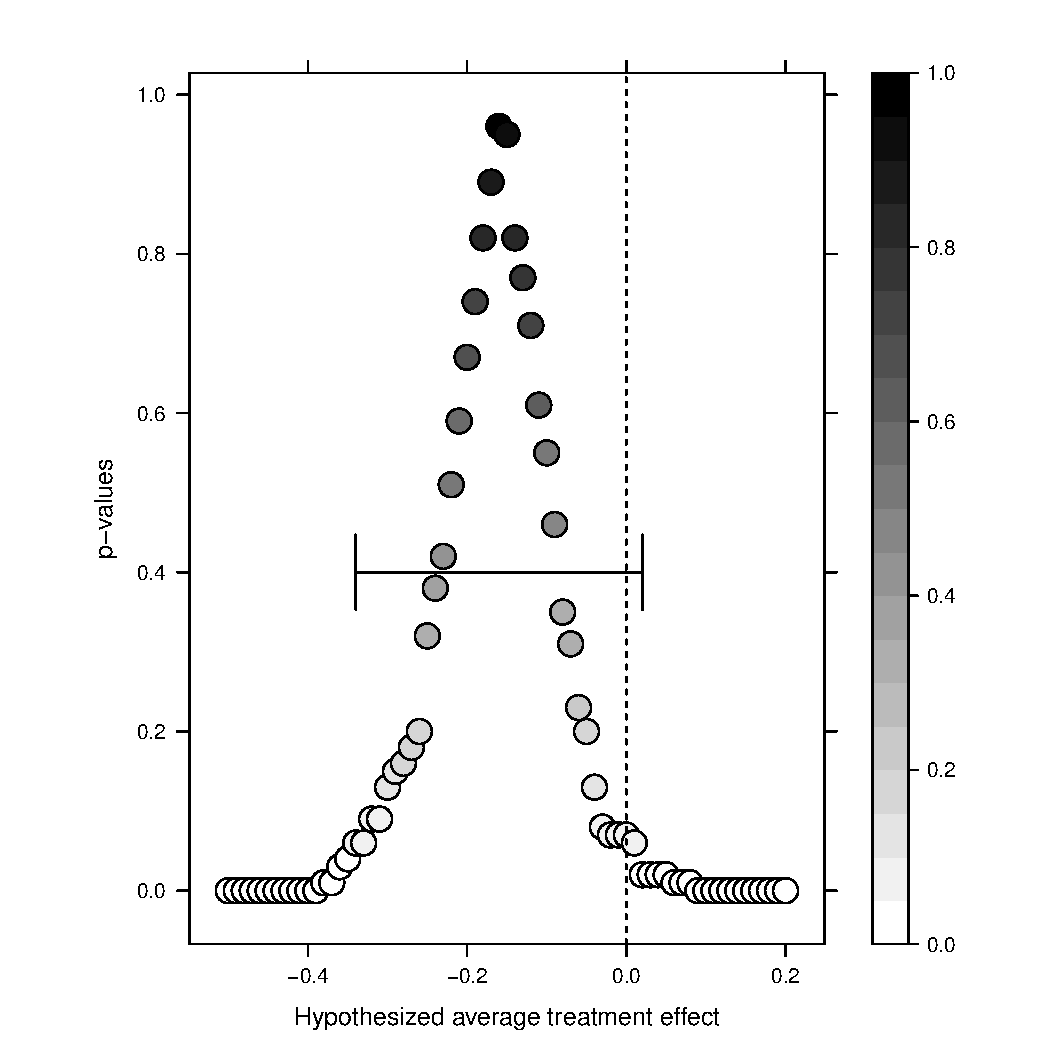
\includegraphics[height=5cm]{images/CoppockJEPS_figure1a.pdf}
\caption{Figure 1}
\end{figure}


Figure 2 shows the heterogeneous effects of treatment. X-axis represents hypothesized effects in higher-support districts as against the hypothesized effects in lower-support districts on Y-axis. Once again, the colour scale indicates the p-value for each pair of hypotheses. Darker region indicates a higher p-value. We observe maximum p-value at effect values (0.05, -0.37) in higher-support and lower-support regions respectively.


\begin{figure}[H]
\centering
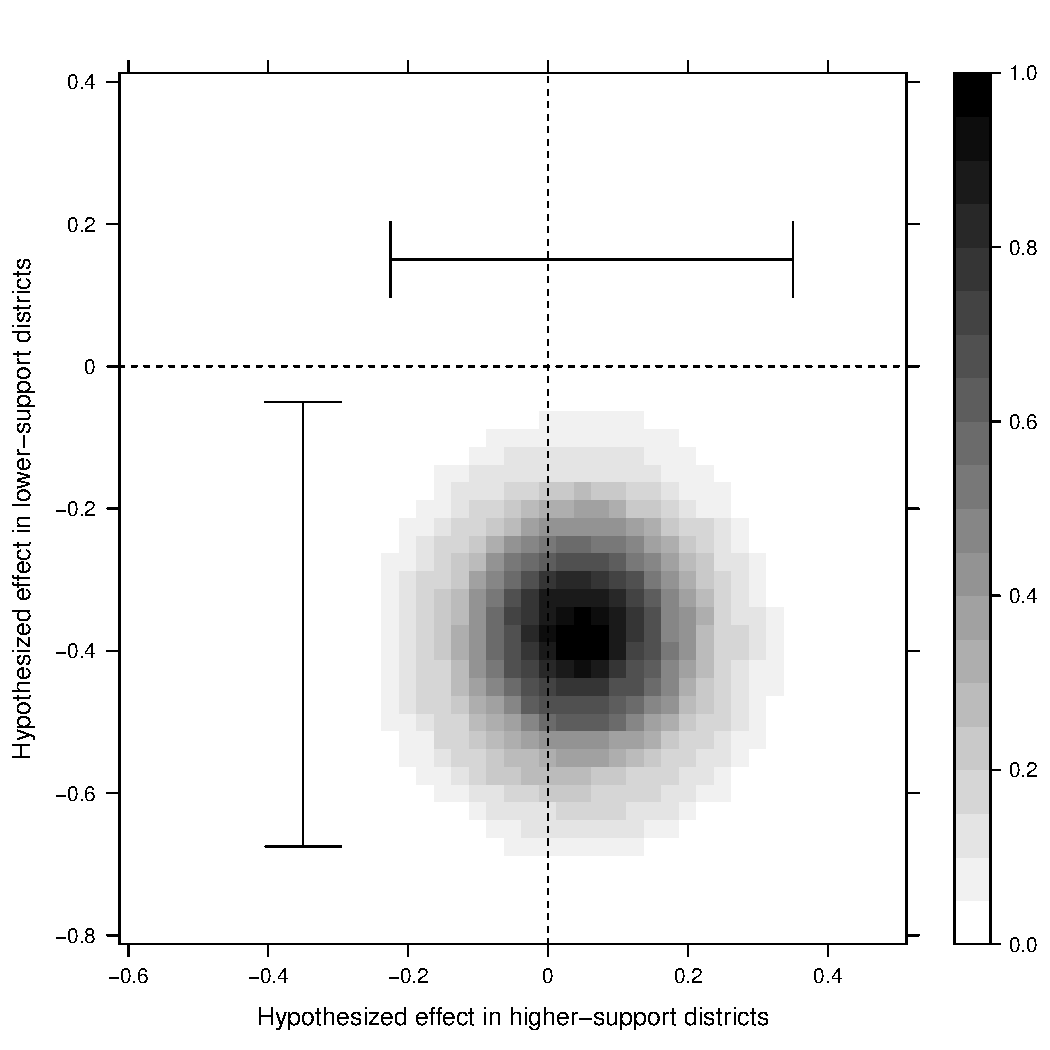
\includegraphics[height=5cm]{images/CoppockJEPS_figure1b.pdf}
\caption{Figure 1}
\end{figure}



Present results when we assume some form of interference \\
Explore how alternative assumptions regarding interference change results



\subsection{tasks}
\begin{itemize}
\item Replicate Bergan. (SP)
\item Find other network data for the New Mexico legislature. (BD)
\item Geography and ideology data for New Hampshire (BD)
\item Produce cosponsorship, ideology and geography estimates for both Bergan and Nickerson (SP \& BD)
\item For at least two spreading models (SP \& BD)
\item Replicate Nyhan (SP)
\end{itemize}


Records of standing committee membership in the 16 standing committees in place during the 2008 regular session was obtained from the New Mexico Legislative Council Service Librarian. 

\begin{figure}
\centering
\begin{tabular}{cc}
{\bf Geographic Network} & {\bf Committee Network (>1 in common)}\\
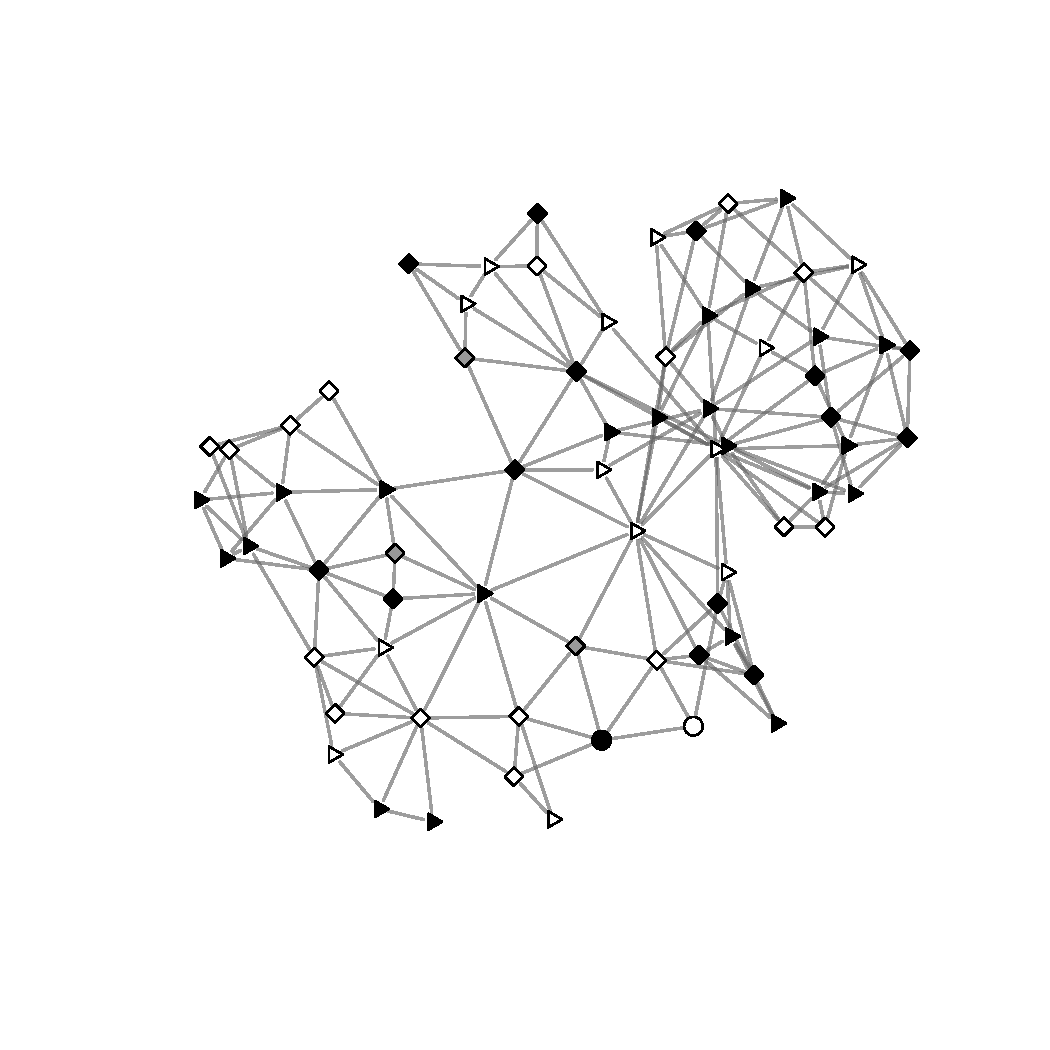
\includegraphics[scale=.55, clip=true,trim =2cm 2cm 2cm 2cm ]{./images/coppock_geographic_net.pdf} & 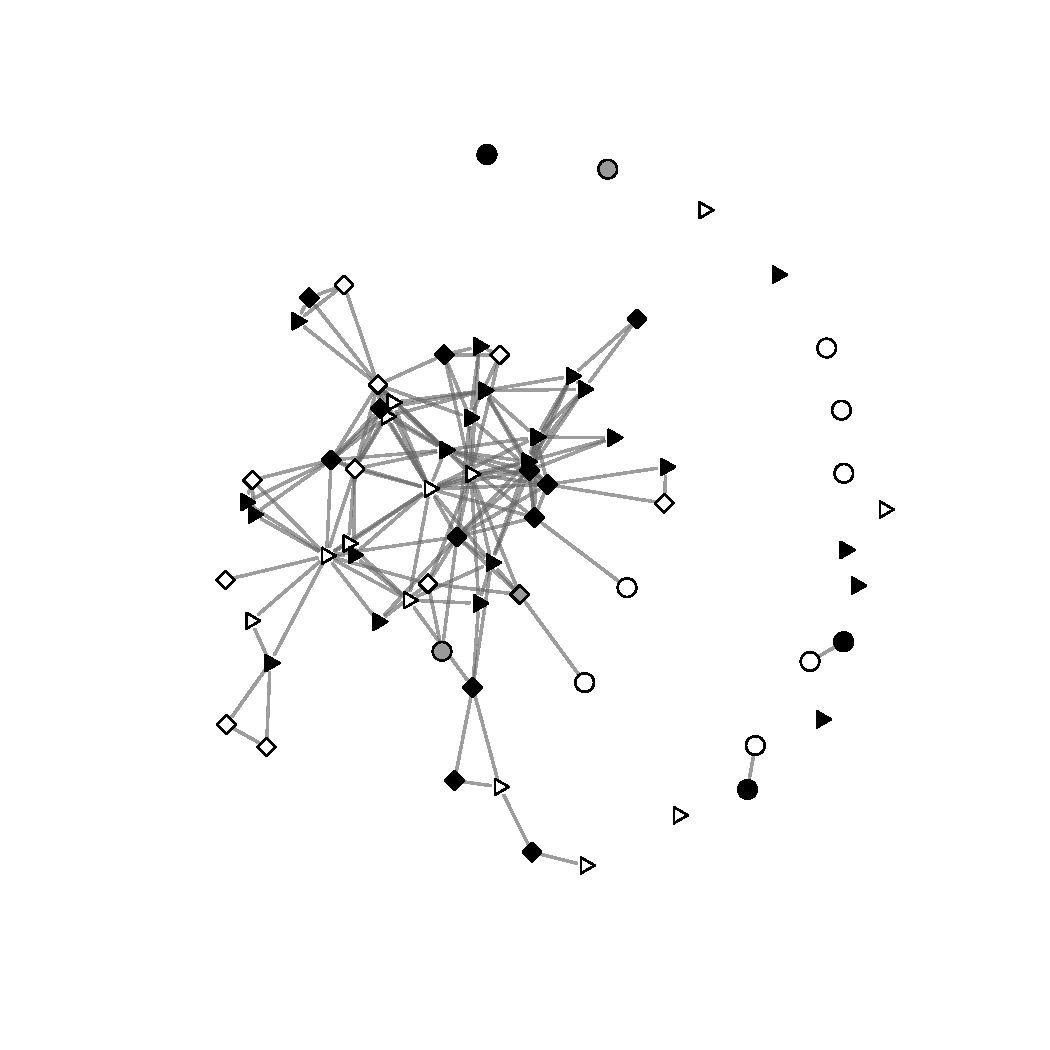
\includegraphics[scale=.55, clip=true,trim =2cm 2cm 2cm 2cm]{./images/nm_committee_net.pdf} \\ 
\end{tabular}
{\bf Ideological Network (top 5\%)} \\
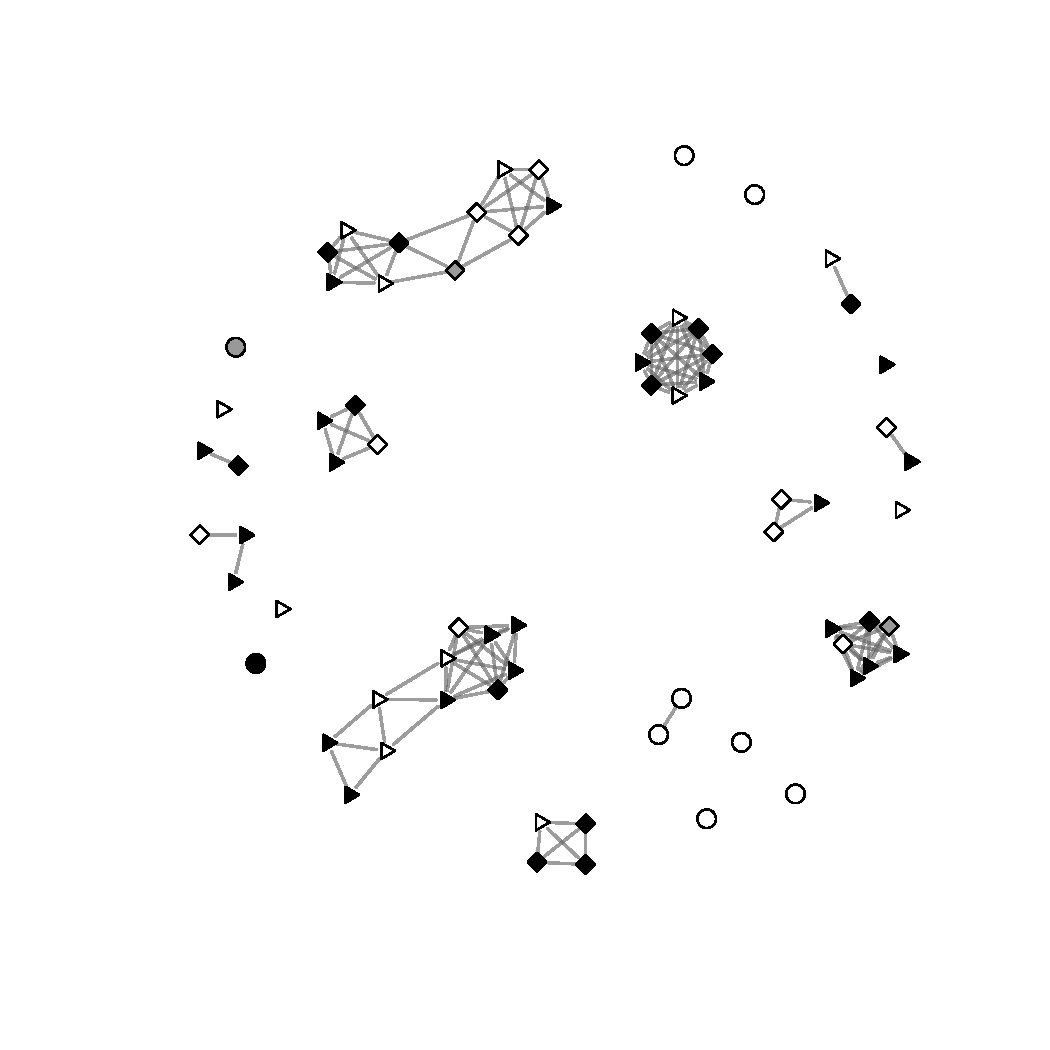
\includegraphics[scale=.55, clip=true,trim =2cm 2cm 2cm 2cm]{./images/coppock_ideological_net.pdf}
\caption{Different networks among New Mexico legislators. Colors denote outcome: black means voted with district, gray means abstained, white means voted against. Shape denotes treatment status. Triangles are treated. Squares are adjacent to treated. Circles are isolated from treatment}
\label{fig:nh-nets}
\end{figure}




%===================References======================
\clearpage
\bibliographystyle{apsr}
\bibliography{cause_and_networks}



\end{document}
